\documentclass{beamer}
%\usepackage[T1]{fontenc}
\usepackage[utf8]{inputenc}
%\usepackage{lmodern}  % Use the Latin Modern font family

\usepackage{latexsym,amsmath,xcolor,bm, amssymb, color, tikz, graphicx, amsthm, mathtools}
\usepackage{algorithm}
\usepackage{algorithmic}
\usepackage{hyperref}
\usepackage{float}     
\usepackage{CJKutf8}
\usepackage{multicol}

\DeclareMathOperator*{\argmax}{arg\,max}
\DeclareMathOperator*{\argmin}{arg\,min}
\DeclareMathOperator{\sign}{sign}
\DeclareMathOperator{\Tr}{Tr}

\makeatletter
\DeclareRobustCommand\onedot{\futurelet\@let@token\@onedot}
\def\@onedot{\ifx\@let@token.\else.\null\fi\xspace}
\def\eg{\emph{e.g}\onedot} 
\def\Eg{\emph{E.g}\onedot}
\def\ie{\emph{i.e}\onedot} 
\def\Ie{\emph{I.e}\onedot}
\def\cf{\emph{c.f}\onedot} 
\def\Cf{\emph{C.f}\onedot}
\def\etc{\emph{etc}\onedot} 
\def\vs{\emph{vs}\onedot}
\def\wrt{w.r.t\onedot} 
\def\dof{d.o.f\onedot}
\def\etal{\emph{et al}\onedot}
\makeatother


\usetheme{Madrid}
\useinnertheme{circles}


\definecolor{ColorUNR}{HTML}{990077} 
\usecolortheme[named=ColorUNR]{structure}
%\usecolortheme[named=ColorUNR]{exampleblock}

%\setbeamertemplate{blocks}[rounded][shadow=true]
%\setbeamercolor{block body}{fg=black,bg=white}



%------------------------------------------------------------
%This block of code defines the information to appear in the
%Title page
\title %optional
{Inauguración del TC}

%\subtitle{(Subtitulo de la Clase)}

%\subtitle{with applications to persuation and lie production}
% \author % (optional)
% {Author Name}

%\author[Matias Ramos]{Matias Ramos}

\institute[]{Universidad Tecnológica Nacional - Facultad Regional Santa Fe}
\date[TC 2024]{Training Camp 2024}
\titlegraphic{
\includegraphics[clip,height=2cm,keepaspectratio]{logos/tcarg.jpeg}}

%End of title page configuration block
%------------------------------------------------------------


%------------------------------------------------------------
%The next block of commands puts the table of contents at the 
%beginning of each section and highlights the current section:
\AtBeginSection[]
{
  \begin{frame}
    \frametitle{Temario}
    \tableofcontents[currentsection]
  \end{frame}
}
%------------------------------------------------------------


\begin{document}


%The next statement creates the title page.
\frame{\titlepage}


%------------------------------------------------------------
% Frame de Sponsors, me parece mejor ponerlo al principio
% Antes del índice/contenido

\begin{frame}{Gracias Sponsors!}
    \begin{columns}[t]
        \column{0.5\textwidth}
        \centering
        Organizador\\
        \vspace{0.8cm}
        
\includegraphics[width=0.7\textwidth,keepaspectratio]{logos/UNRlogo.png}
        
\includegraphics[width=0.7\textwidth,keepaspectratio]{logos/FCEIA.png}
        \column{0.5\textwidth}
        \centering
        Diamond\\
        
\includegraphics[width=1\textwidth,keepaspectratio]{logos/GTSlogo.jpeg}
    \end{columns}
    \begin{columns}[t]
        \column{1.0\textwidth}
        \centering
        Gold\\
        \begin{minipage}{0.5\textwidth}
            \centering
            
\includegraphics[width=0.4\textwidth,keepaspectratio]{logos/avature.jpg}
        \end{minipage}%
        \begin{minipage}{0.5\textwidth}
            \centering
            
\includegraphics[width=0.4\textwidth,keepaspectratio]{logos/Acc_Logo_Black_Purple_RGB.png}
        \end{minipage}
    \end{columns}
\end{frame}


%---------------------------------------------------------
%This block of code is for the table of contents after
%the title page
\begin{frame}
\frametitle{Temario}
\tableofcontents
\end{frame}
%---------------------------------------------------------


\section{Un poco de historia del TC}

\begin{frame}{Los comienzos}
    
    \begin{itemize}
        \item El Training Camp Argentina nace en 2010, inspirandose en los entrenamientos que venian realizandose en Rusia, y que habia comenzado el año anterior en Brasil.
        \item Ese primer Training Camp duro 5 días, y se realizo en la UBA.
        \item Ese primer año solo participaron equipos de Argentina.
        \item Ya al año siguiente se sumaron equipos de países vecinos.
    \end{itemize}
\end{frame}

\begin{frame}{Sedes}
    \begin{itemize}
        \item 2010 - FCEN UBA, Ciudad Autónoma de Buenos Aires
        \item 2011 - FCEN UBA, Ciudad Autónoma de Buenos Aires
        \item 2012 - FAMAF UNC, Ciudad de Cordoba, Cordoba
        \item 2013 - UNLP, La Plata, Provincia de Buenos Aires
        \item 2014 - FCEN UBA, Ciudad Autónoma de Buenos Aires
        \item 2015 - UNS, Bahia Blanca, Provincia de Buenos Aires
        \item 2016 - UNComa, Ciudad de Neuquén, Neuquén
        \item 2017 - UNSAM, San Martin, AMBA, Provincia de Buenos Aires
        \item 2018 - FCEN UBA, Ciudad Autónoma de Buenos Aires
        \item 2019 - FAMAF UNC, Ciudad de Cordoba, Cordoba
        \item 2020 - Remoto
        \item 2021 - Remoto
        \item 2022 - Remoto
        \item 2023 - UNLaM, La Matanza, AMBA, Provincia de Buenos Aires
        \item $\bm{2024 - UNR, Rosario, Santa Fe}$
    \end{itemize}
\end{frame}

\section{Datos del TC}
\begin{frame}{Datos}
    \begin{itemize}
        \item En estas dos semanas van a resolver entre 35-70 problemas.
        \item Desde el 2010, el 95\% de los finalistas argentinos, participaron del TC Argentina.
        \item De los últimos 5 equipos Latam Champions, 4 participaron del TC Argentina.
    \end{itemize}
\end{frame}

\section{Universidad Nacional de Rosario}
\begin{frame}{UNR en ICPC}
    \begin{columns}[t]
        \column{0.5\textwidth}
        \centering
        2015\\
        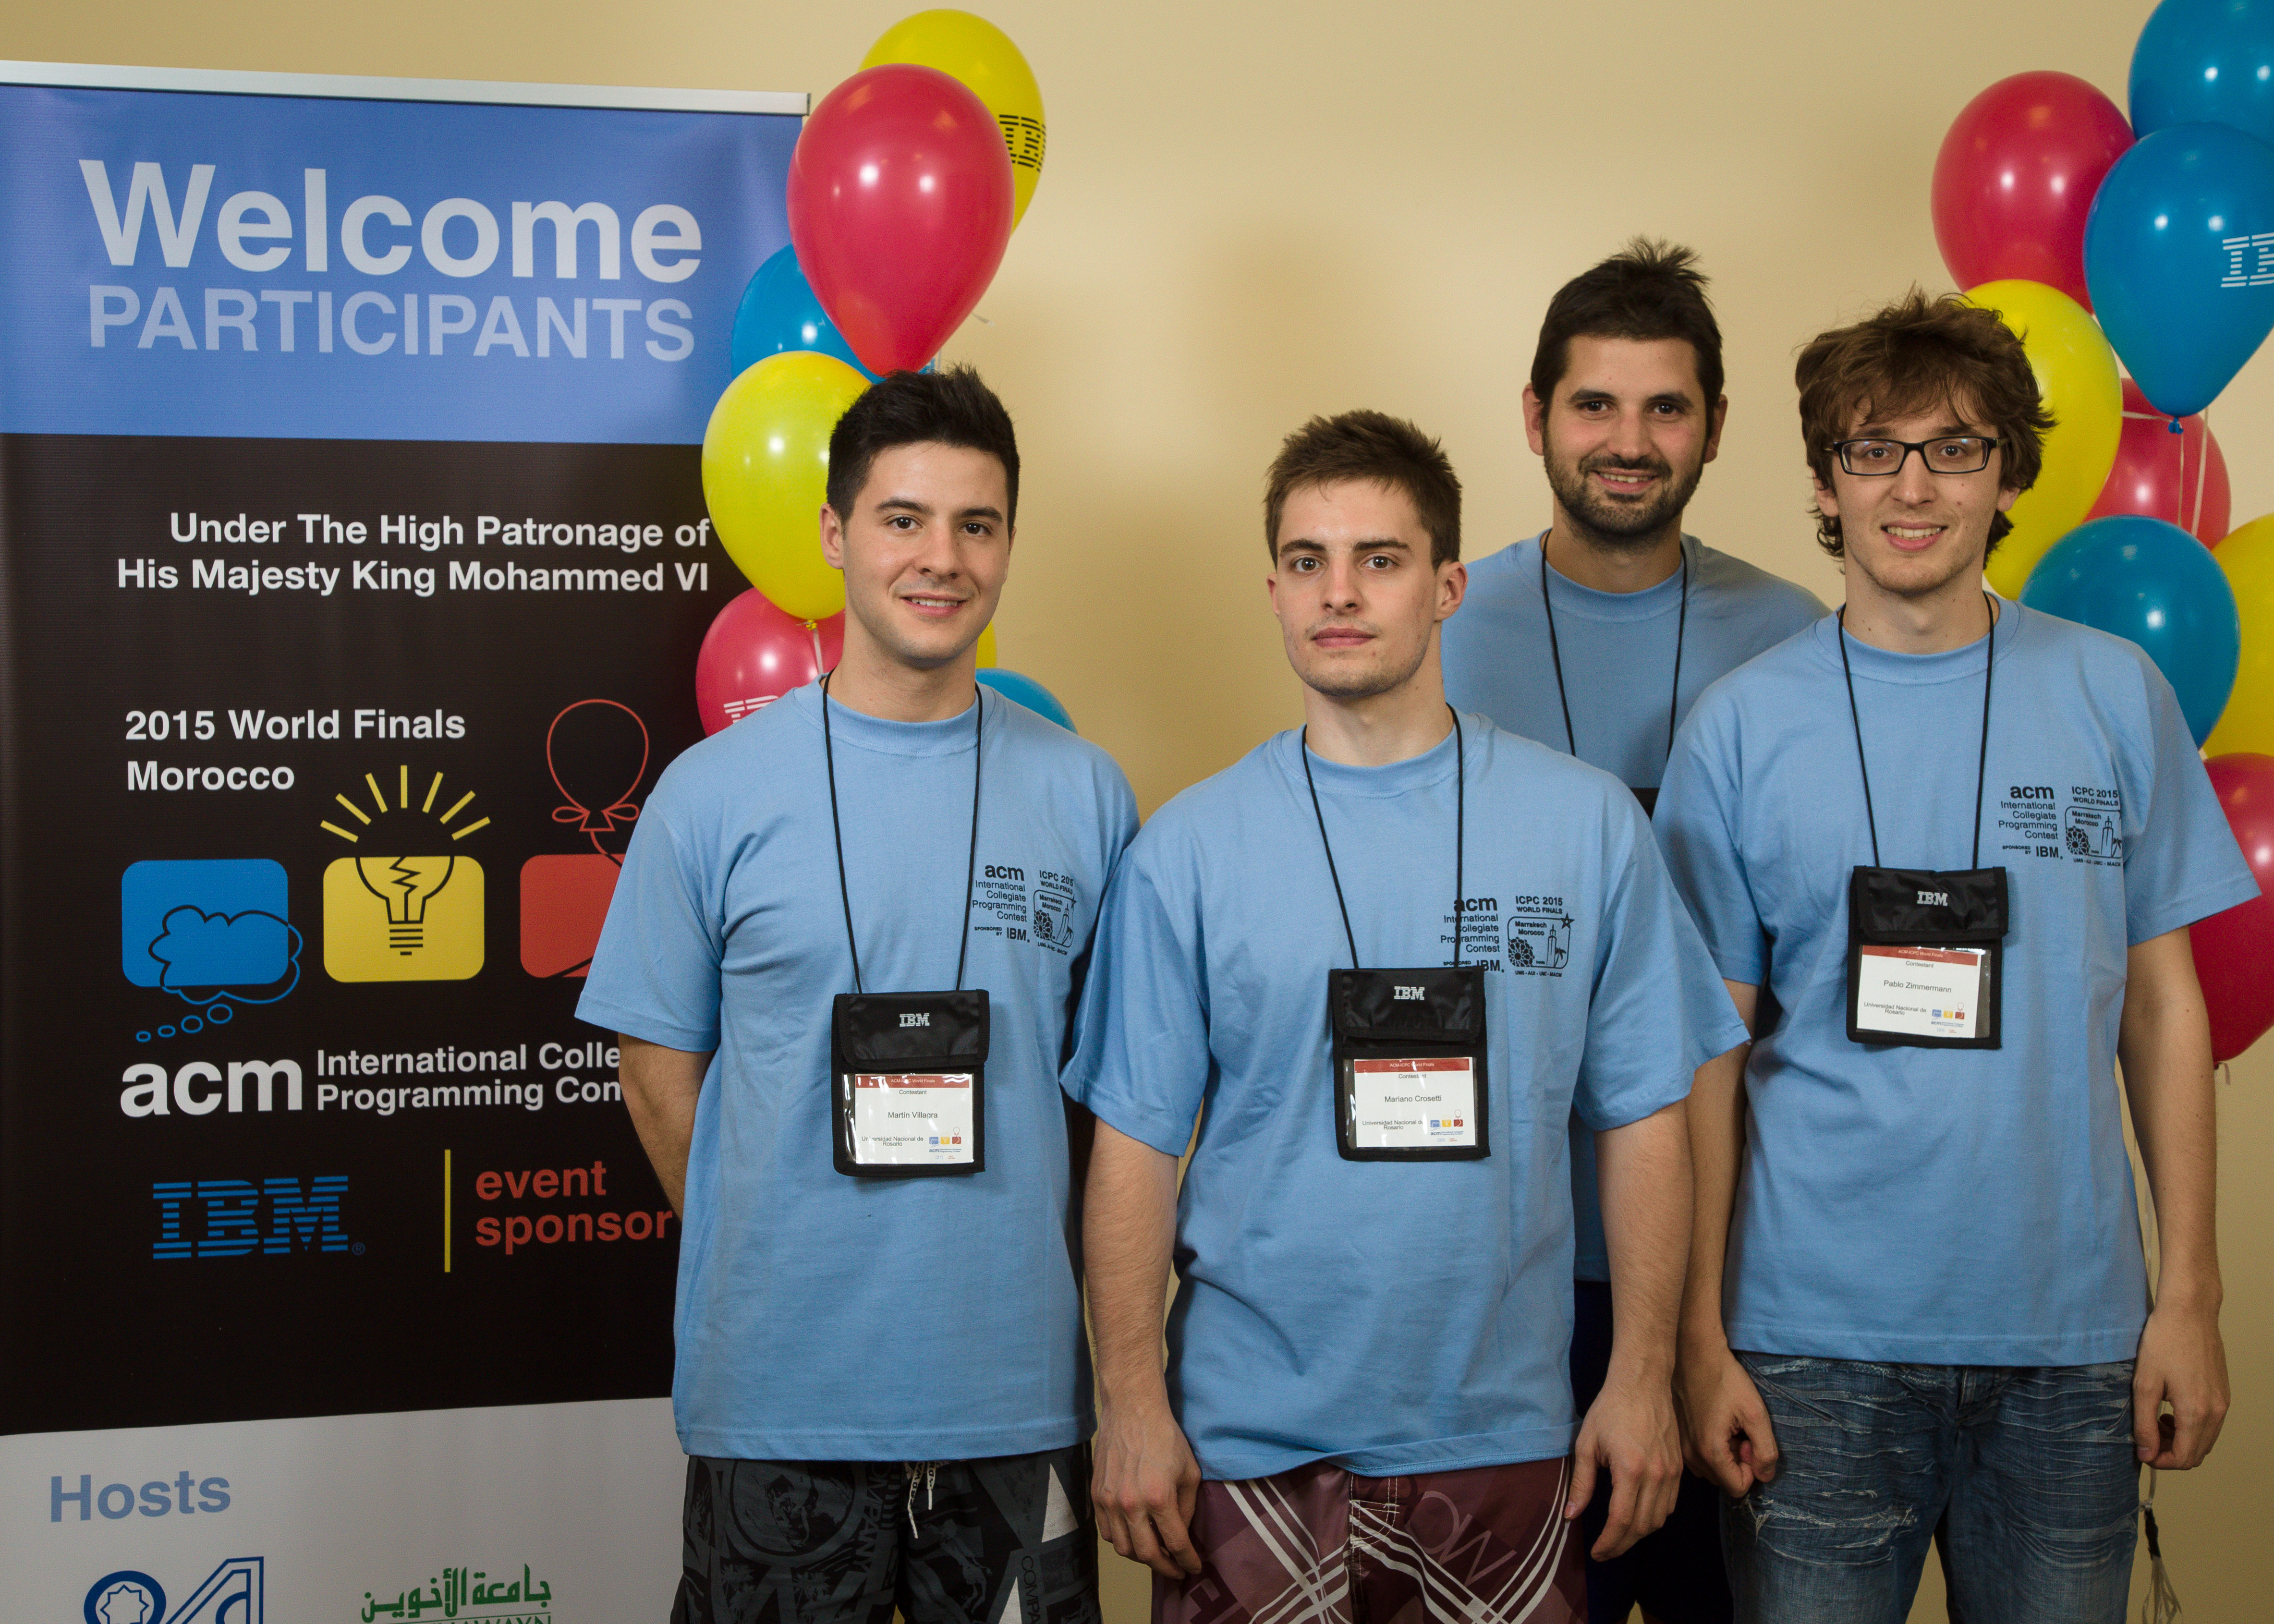
\includegraphics[width=1\textwidth]{img/2015_marruecos.jpg}
        \column{0.5\textwidth}
        \centering
        2016\\
        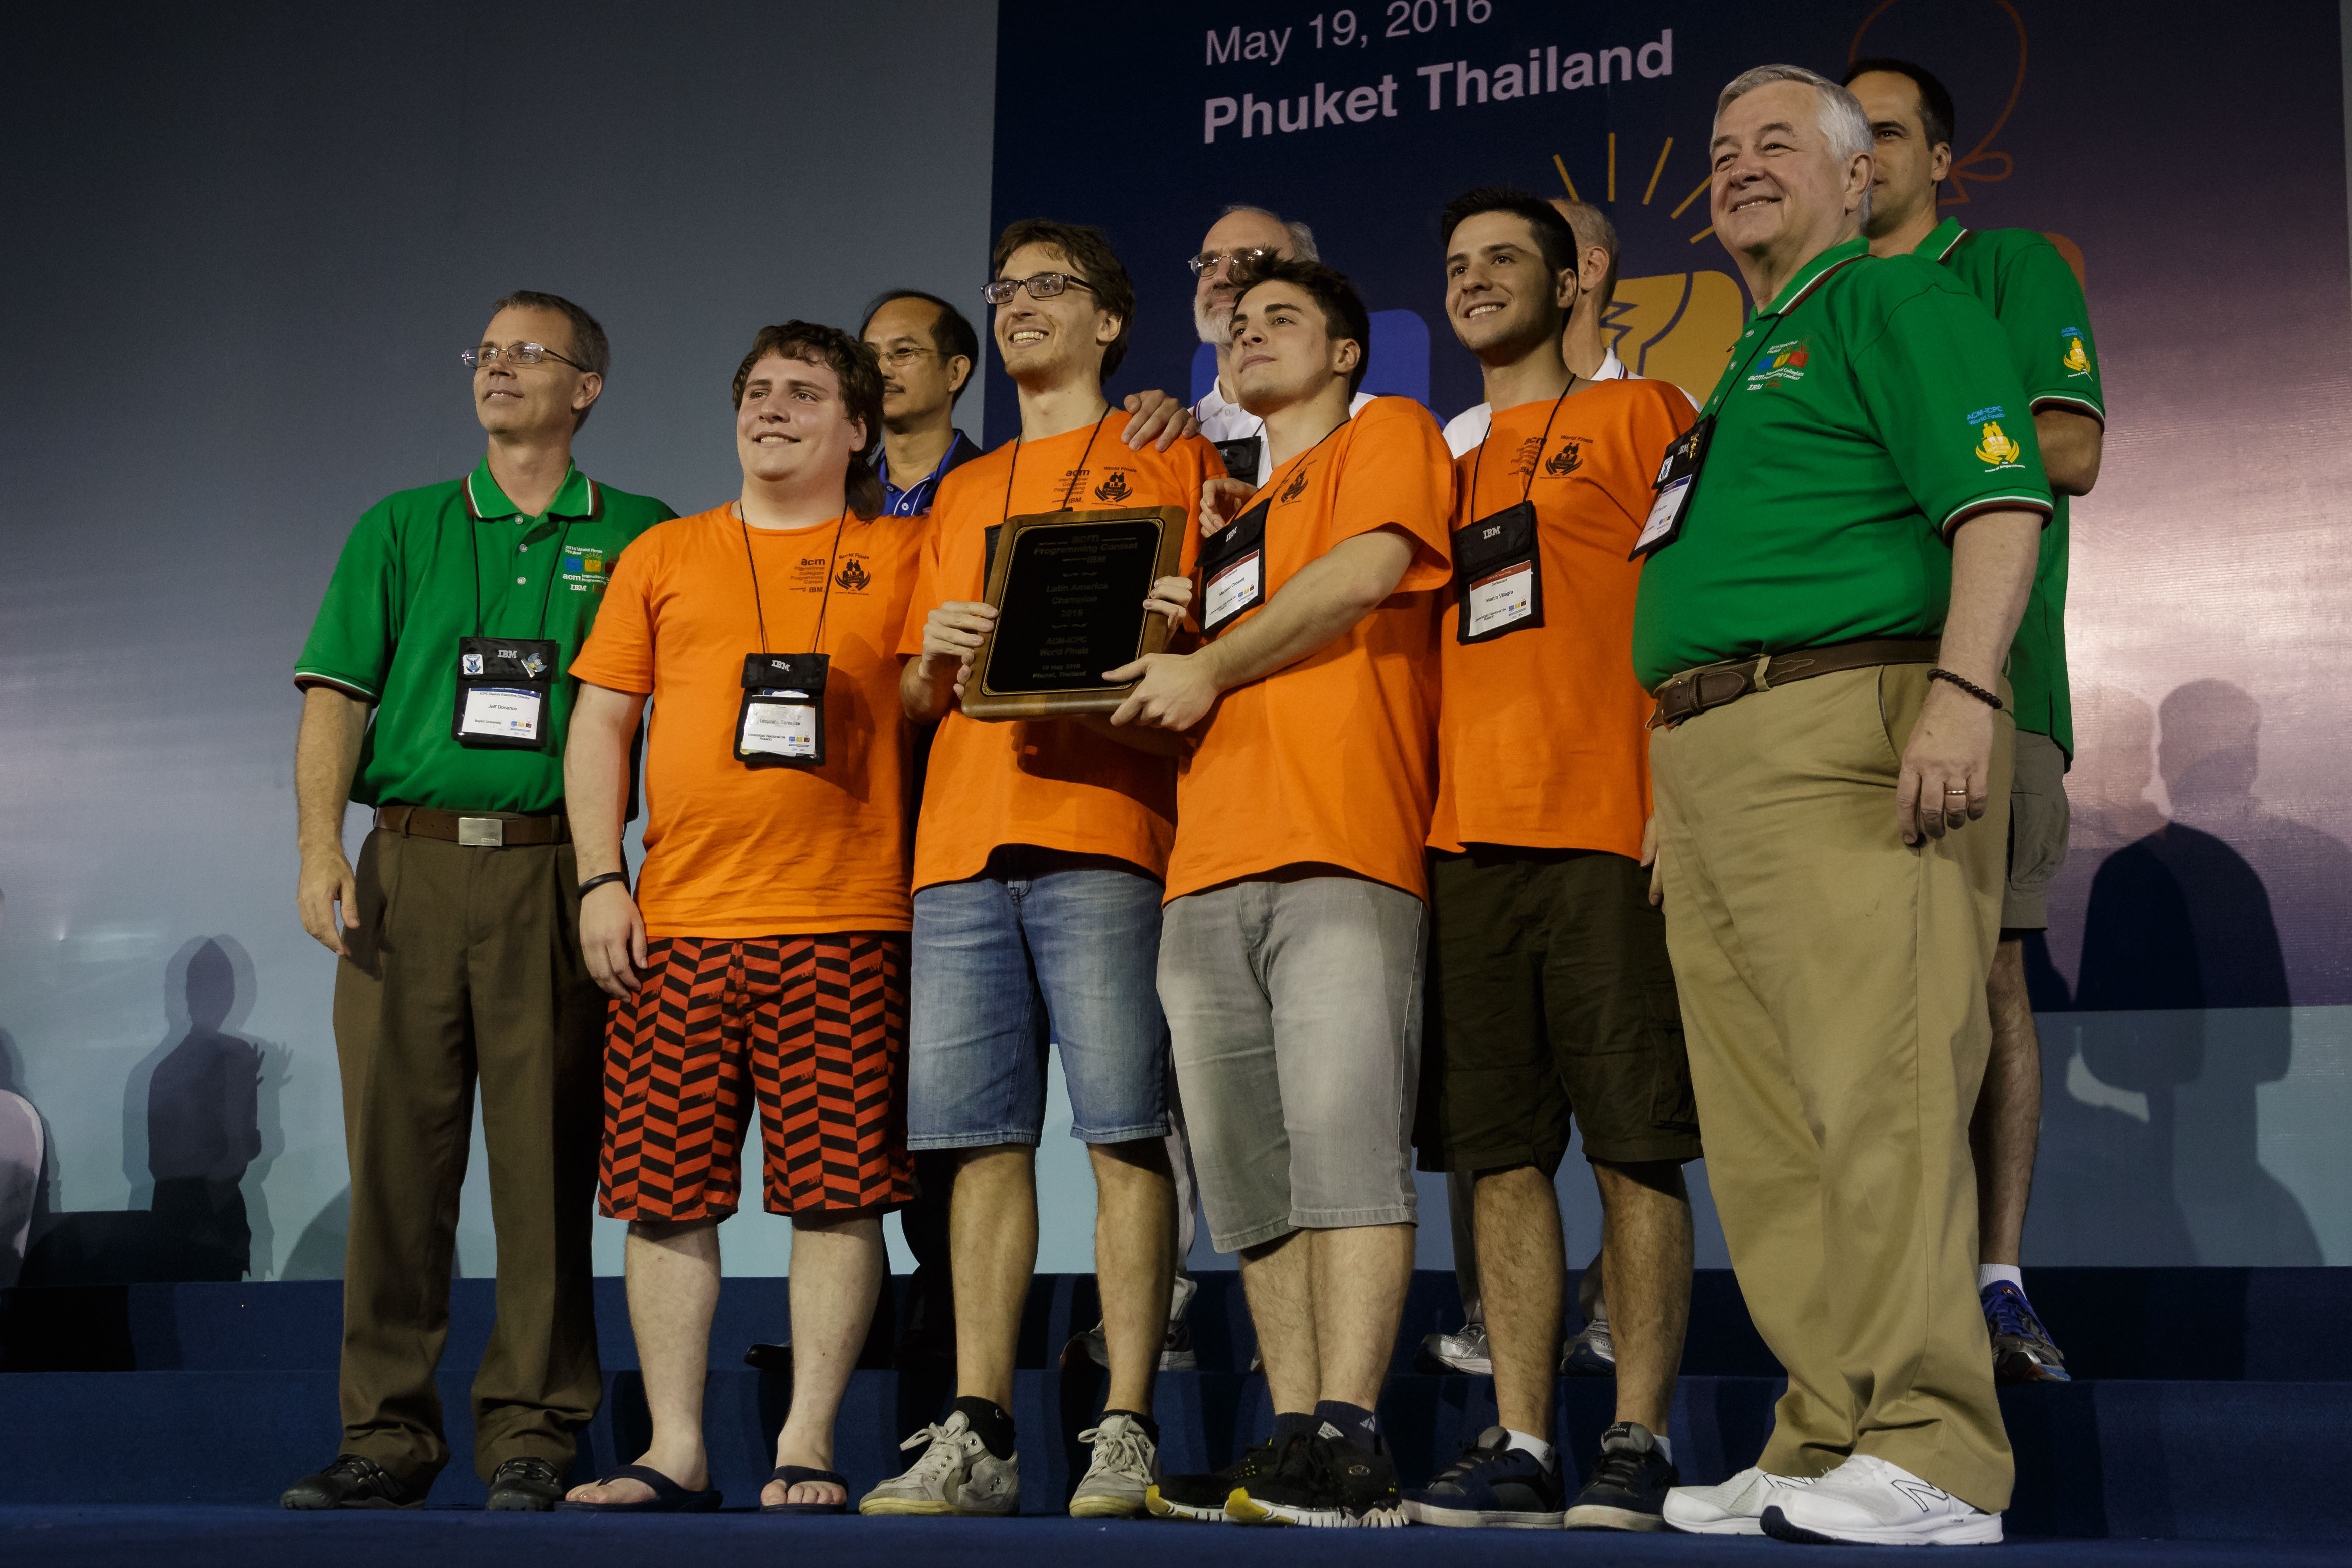
\includegraphics[width=1\textwidth]{img/2016_thailand.jpg}
    \end{columns}
\end{frame}

\begin{frame}{UNR en ICPC}
    \begin{columns}[t]
        \column{0.5\textwidth}
        \centering
        2017\\
        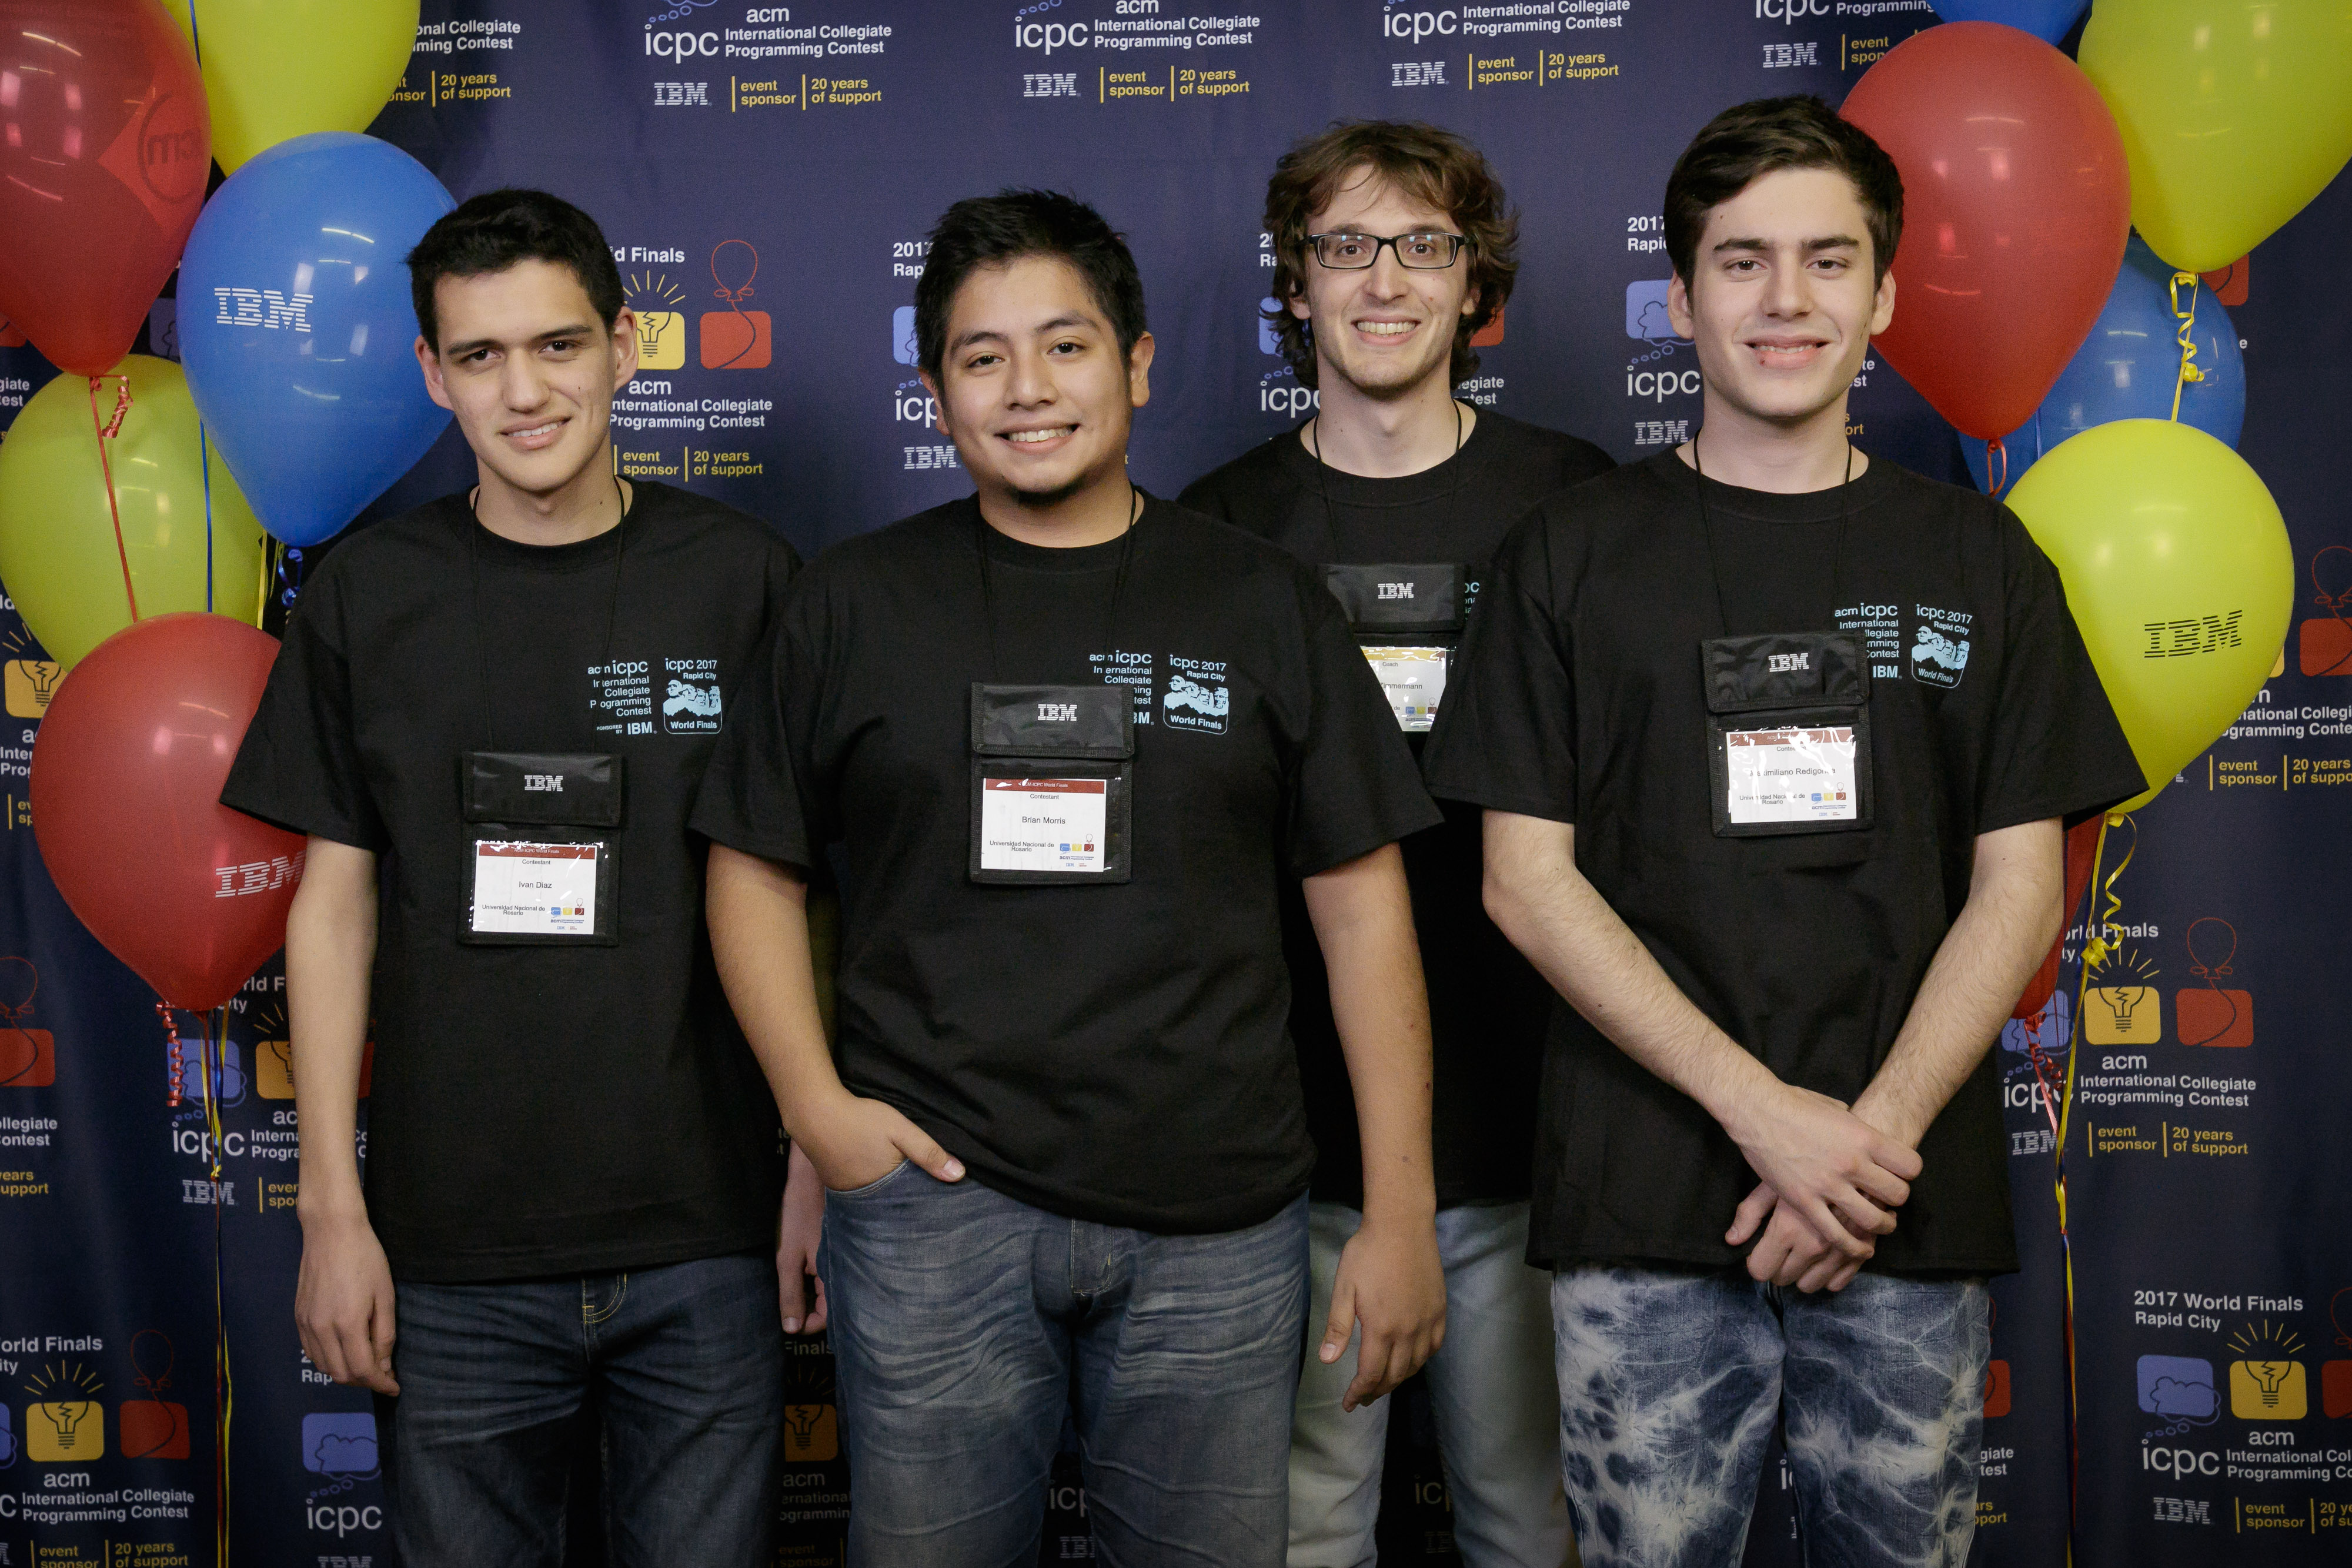
\includegraphics[width=1\textwidth]{img/2017_usa.jpg}
        \column{0.5\textwidth}
        \centering
        2018\\
        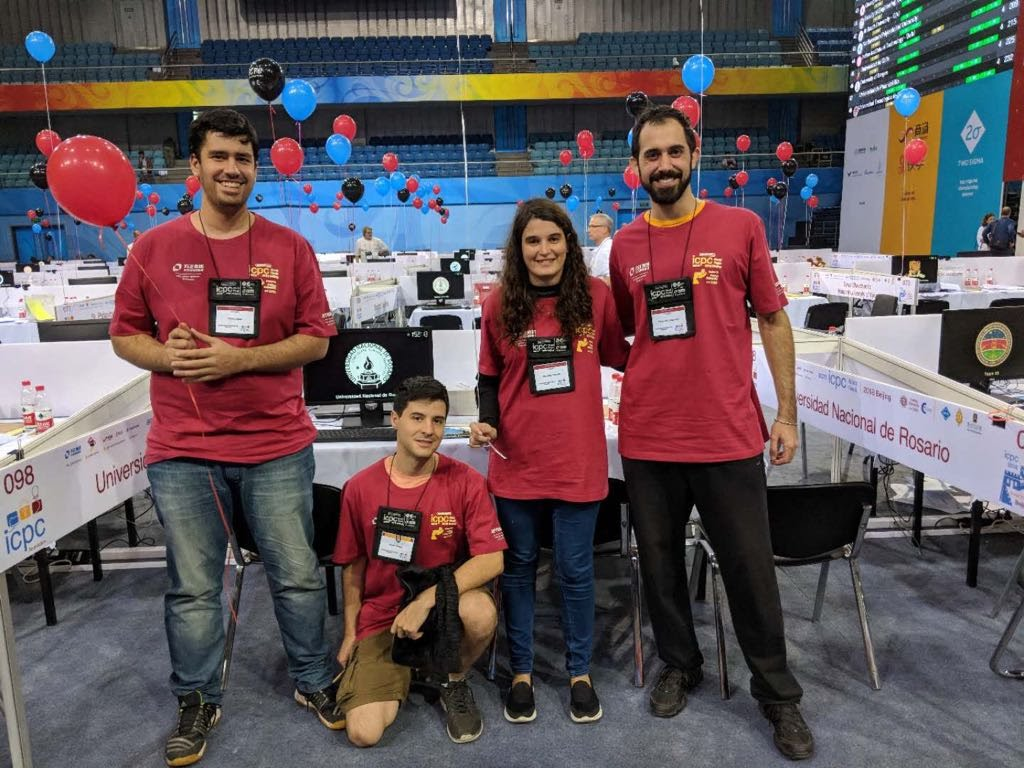
\includegraphics[width=1\textwidth]{img/2018_china.jpeg}
    \end{columns}
\end{frame}

\begin{frame}{UNR en ICPC}
    \begin{columns}[t]
        \column{0.5\textwidth}
        \centering
        2019\\
        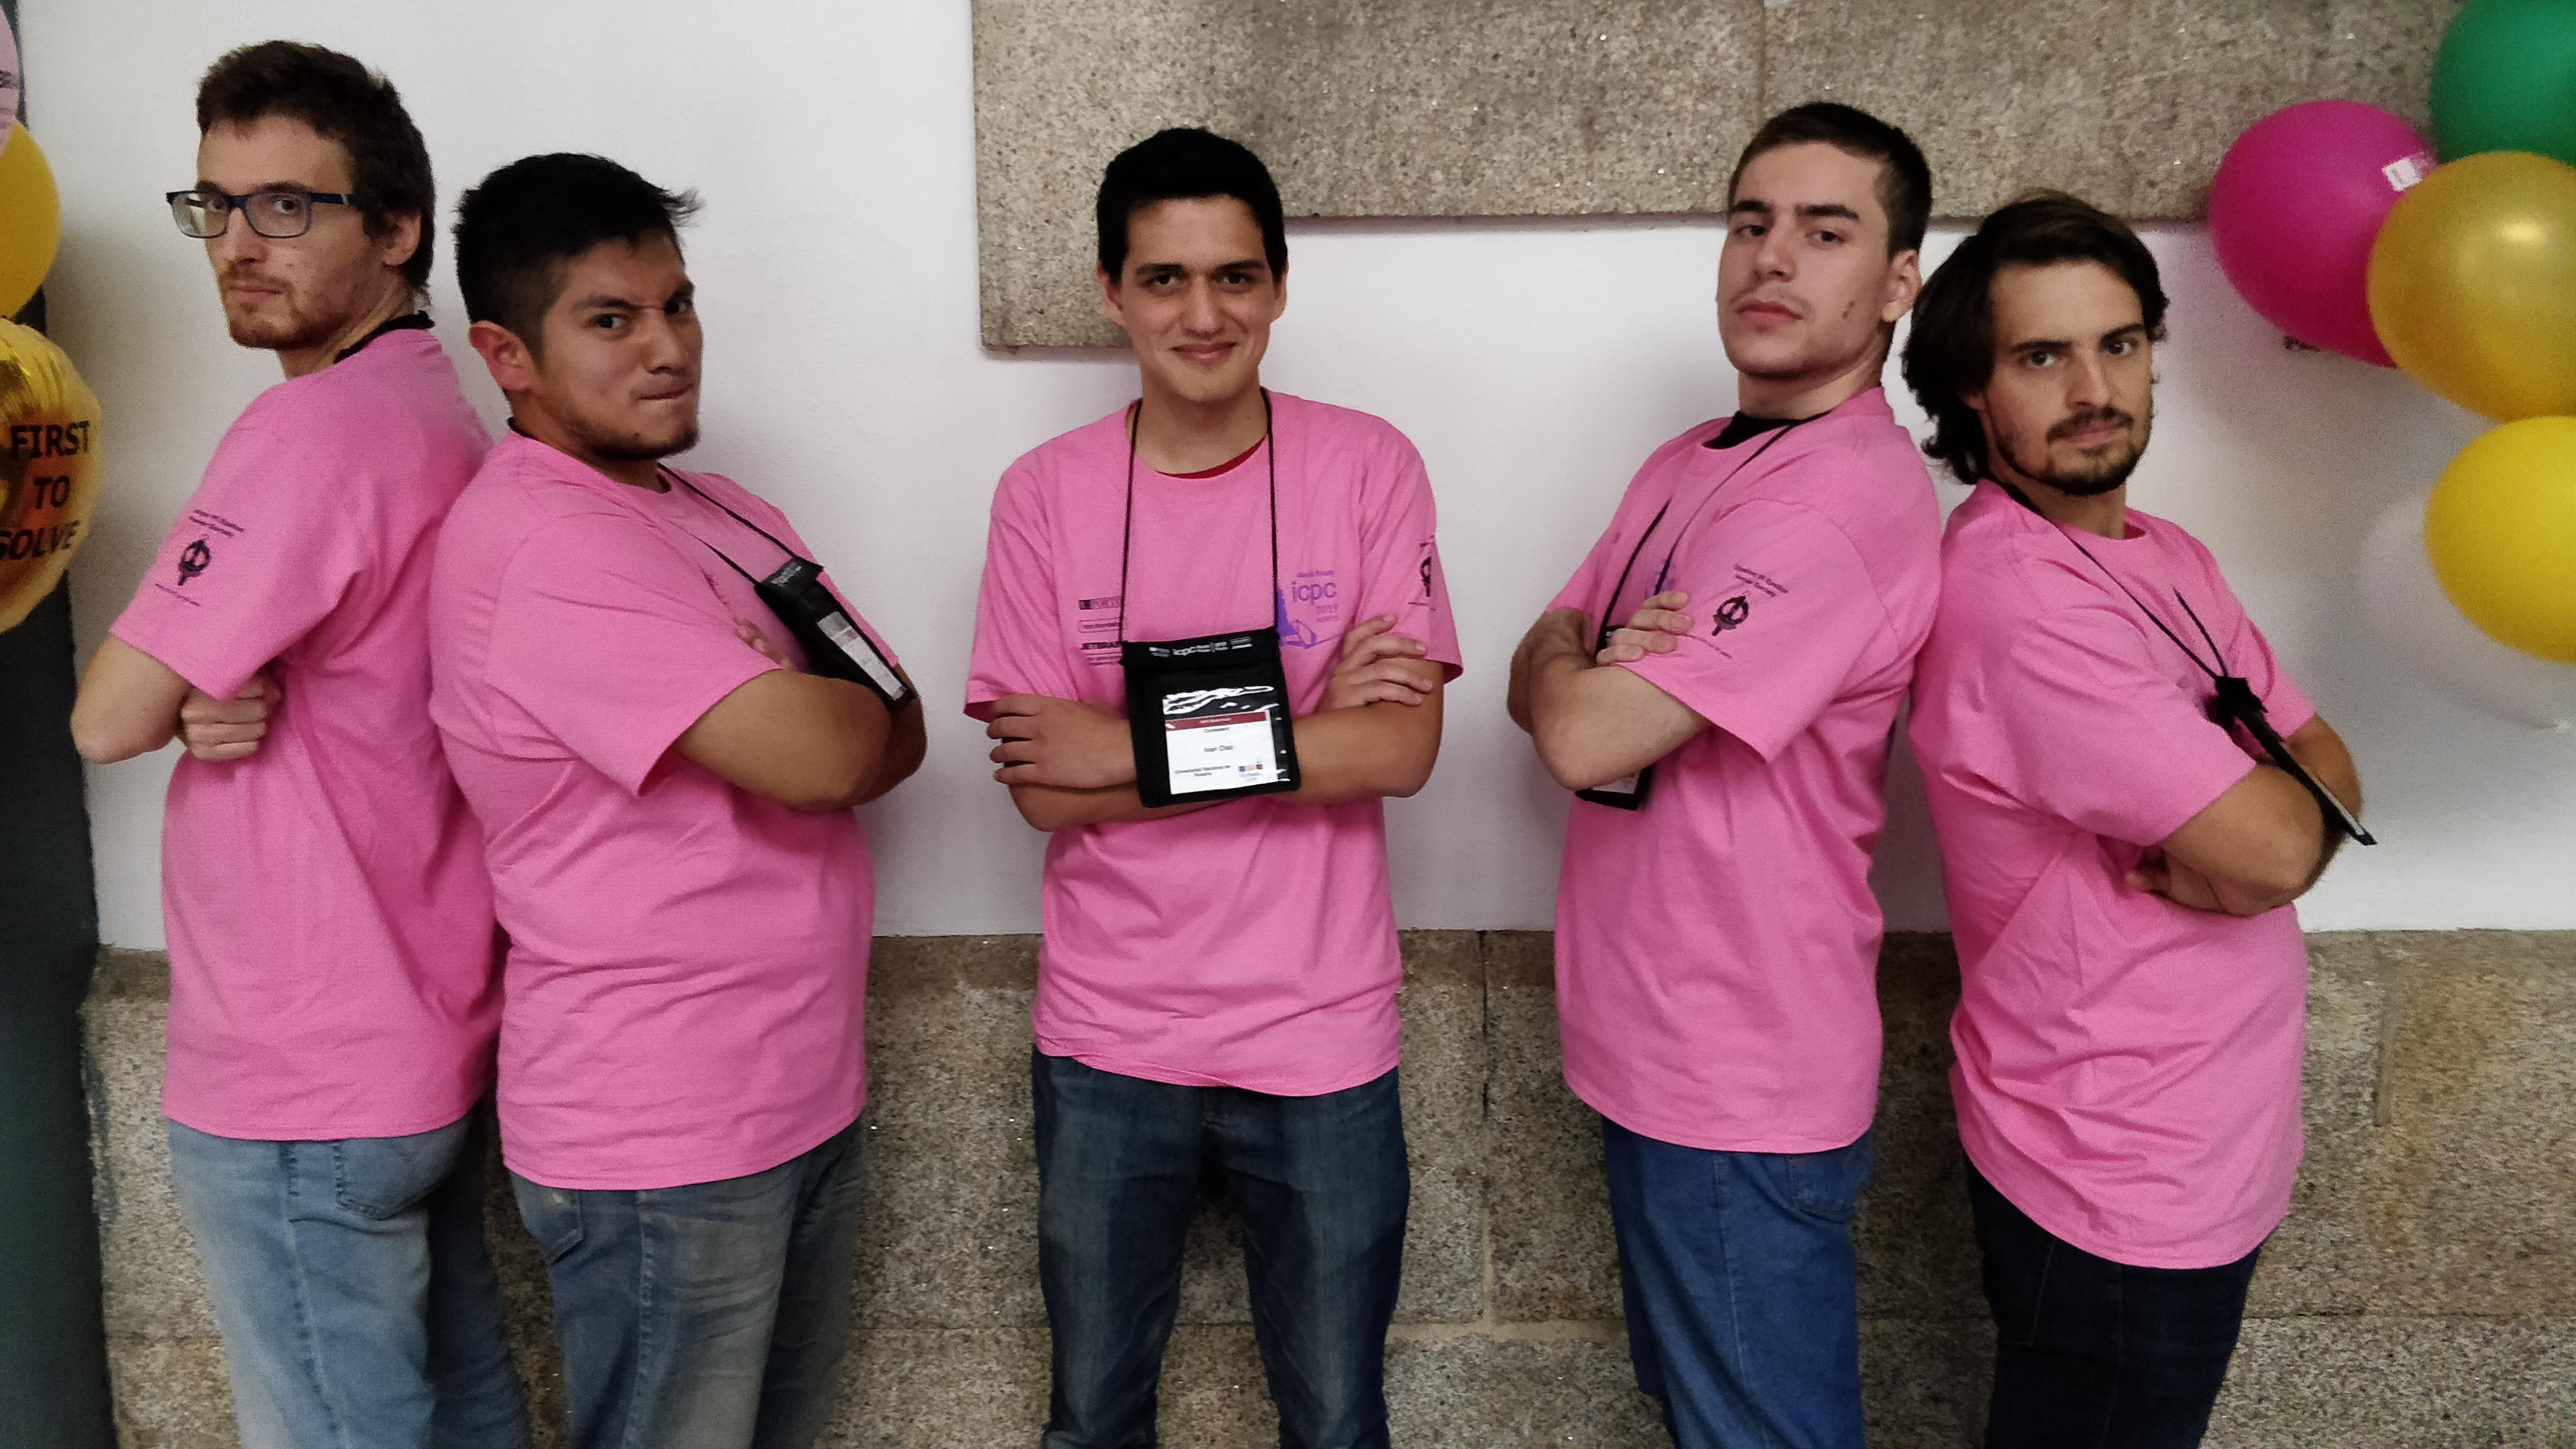
\includegraphics[width=1\textwidth]{img/2019_porto.jpg}
        \column{0.5\textwidth}
        \centering
        2023\\
        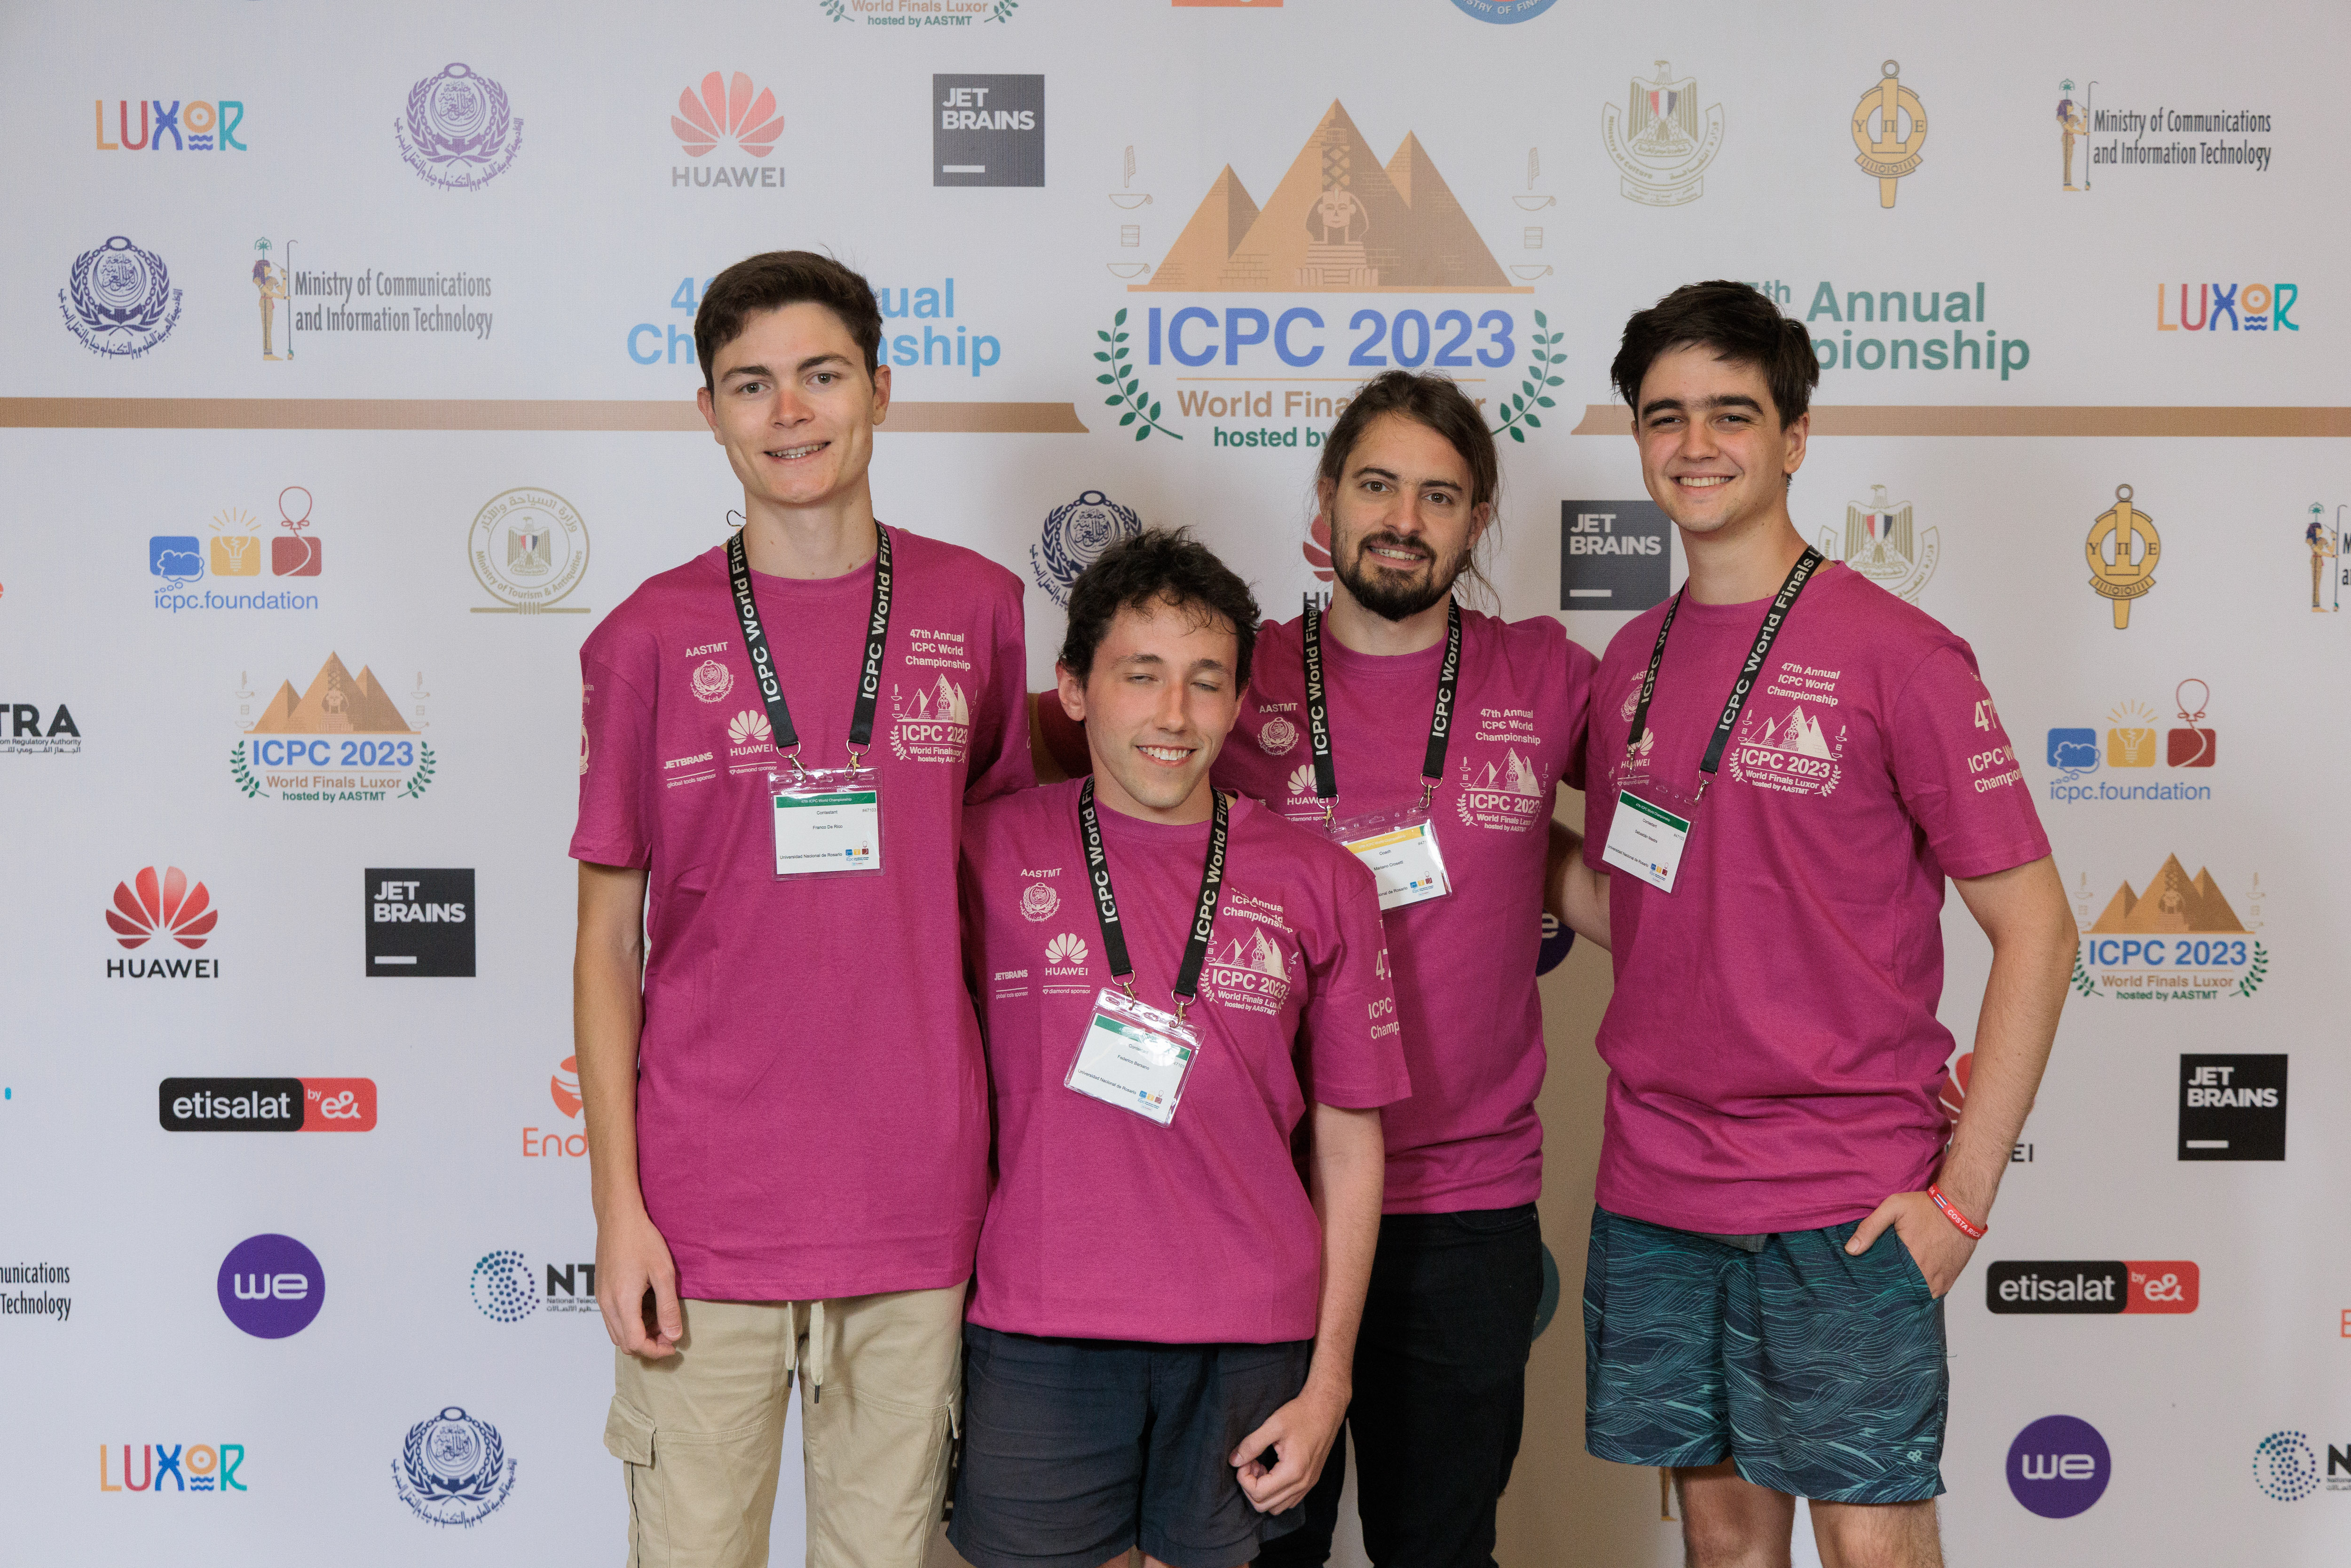
\includegraphics[width=1\textwidth]{img/2023_egipt.jpg}
    \end{columns}
\end{frame}

\begin{frame}{Palabras}
    \begin{columns}[t]
        \column{0.5\textwidth}
        \centering
        
\includegraphics[width=1\textwidth]{logos/UNRlogo.png}
        \column{0.5\textwidth}
        \centering
        
\includegraphics[width=1\textwidth]{logos/FCEIA.png}
    \end{columns}
\end{frame}

\section{GTS - Sponsor Diamond}
    
\begin{frame}{GTS}
    \centering
    
\includegraphics[height=8cm,keepaspectratio]{logos/GTSlogo.jpeg}
\end{frame}


\begin{frame}{Gracias}
    \centering
    Gracias a todos por venir.\\
    Suerte en la competencia de hoy!
\end{frame}


\end{document}